\section{POI, Query and Path}
\label{sec:method}

\begin{figure*}
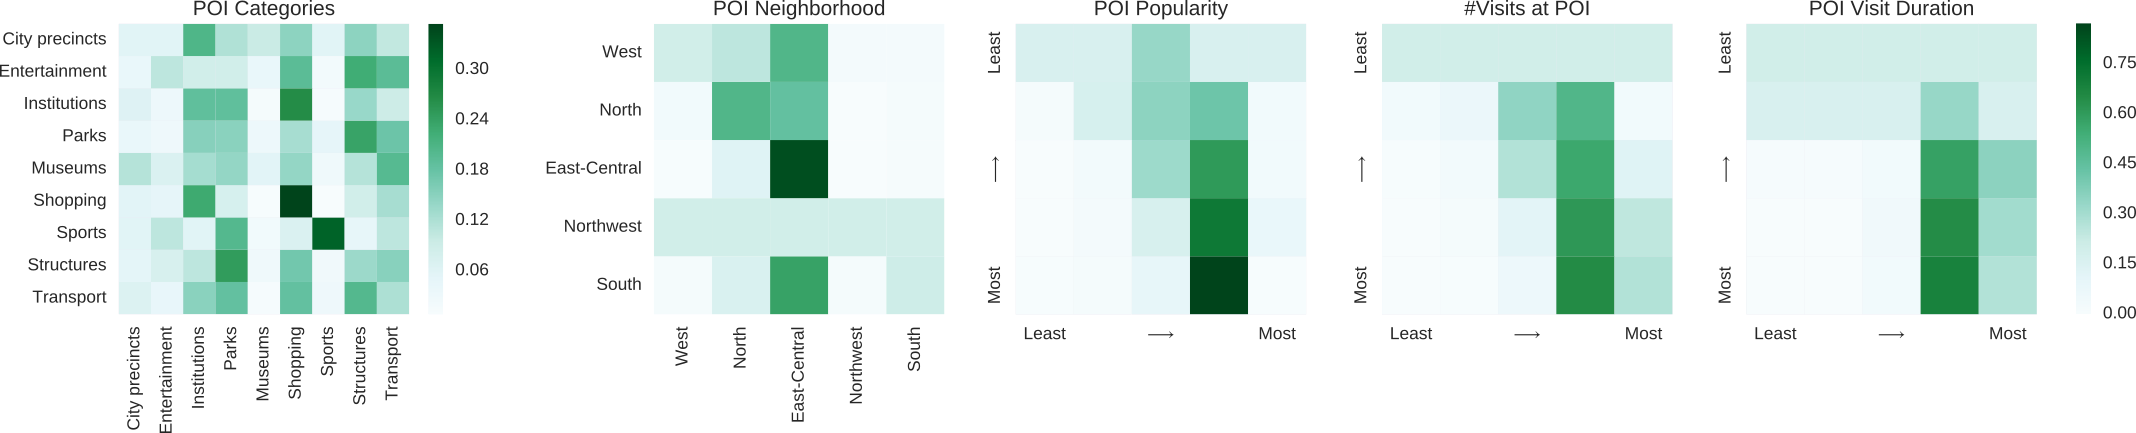
\includegraphics[width=\textwidth]{fig/poi_transmat.png}
\caption{Transition matrices for $5$ individual POI features (Melbourne)}
\label{fig:transmat}
\end{figure*}


We would like to recommend a particular tour such that the user will visit a sequence of points of interests (POIs), denoted $p_1, \ldots, p_L$, that maximises utility. We are given the desired start ($p_1=p_s$) and end point ($p_L=p_e$), and an associated number $L$ of POIs desired, from which we propose a trajectory through the city. In Figure~\ref{fig:problems}, an example tour is shown in blue, which starts at the POI denoted as a grey star, visits two intermediate POIs, and terminates on the fourth POI denoted as a flag. The tour of length 3 can be modelled as a sequence of directed edges in a graph containing POIs in the city as nodes.

The training data consists of a set of tours of varying length in a particular city. We assume that all POIs in the city are visited at least once, and hence can construct a graph with POIs as nodes and potentially multiple directed edges between each pair of nodes. We extract the category, popularity, total number of visits and average visit duration for each POI. The set of categories are shown in figure \ref{fig:poicats} in the appendix, and the popularity is defined as the number of distinct users that visited the POI\cite{ht10}.

As a baseline approach, we recommend the trajectory based on the popularity of POIs only, that is we always suggest the top-$k$ most visited POIs for all visitors given the start and end location. This baseline approach, called \textsc{PoiPopularity}, and its only adaptation to a particular request is to adjust $k$ to match the desired length.

\cheng{I have removed reference to user specific recommendations.}


\subsection{Ranking using the origin and destination}
\label{sec:ranksvm}

\dawei{Features of target POI are already described here.} 

In addition to popularity, we also can rank the recommended POIs based on the other three POI specific features (category, total visits and average duration).
We can learn a ranking of POIs by using rankSVM with linear kernel and $L2$ loss\cite{lranksvm},
\begin{displaymath}
\min_{\mathbf{w_r}} \frac{1}{2} \mathbf{w_r}^T \mathbf{w_r} +
                    C_r \sum_{(p_i, p_j) \in \mathcal{P}}
                    \max \left( 0, 1 - \mathbf{w_r}^T (\mathbf{f}_{p_i} - \mathbf{f}_{p_j}) \right)^2
\end{displaymath}
where $\mathbf{w_r}$ is a vector of parameters,
$C_r > 0$ is the regularization parameter and
$\mathbf{f}_{p_i}$ is the feature vector described below.

Furthermore, since we are constrained by the fact that trajectories have to be of length $L$ and start and end at certain points, we hope to improve the recommendation by using this information.
In other words, using the query $(p_s, p_e, L)$ we can construct new features by contrasting
candidate POIs with $p_s$ and $p_e$.

For each of the POI features above, we construct two new features by taking the difference of
the feature in POI $p$ with $(p_s, p_e)$ respectively.
For the category, we set the feature to $1$ when their categories are the same and $-1$ otherwise.
For popularity, total visits and visit duration, we take the real valued difference.
The distance from POI $p$ to $p_s$ (and $p_e$) is computed using the haversine formula \cite{haversine},
\begin{displaymath}
  d(p, p_s) = 2 R_1 \arcsin \sqrt{ \sin^2 \frac{\Delta \phi}{2} +
    \cos \phi_p \cos \phi_{p_s} \sin^2 \frac{\Delta \lambda}{2} }
\end{displaymath}
where $R_1 = 6371.0088$ km is the mean earth radius \cite{earth_radius},
$\Delta \phi = \phi_p - \phi_{p_s}$, $\Delta \lambda = \lambda_p - \lambda_{p_s}$,
and $\phi_p$, $\lambda_p$ are the latitude and longitude of POI $p$ respectively.
Lastly we also include the required length $L$ of the trajectory as a feature for rankSVM.

For training the rankSVM, the labels are generated using the number of occurrences of
POI $p$ in trajectories grouped by query $(p_s, p_e, L)$,
without counting the occurrence of $p$ when it is the origin or destination POI of a trajectory.
We create another algorithm to recommend trajectory by utilising
the ranking of POIs described above,
the pseudo code of this algorithm, \textsc{PoiRank}, is described in algorithm \ref{alg:poirank}.

\begin{algorithm}
\caption{\textsc{PoiRank}: recommend trajectory by ranking POIs}
%\caption{\textsc{PoiRank}}
\label{alg:poirank}
\begin{algorithmic}[1]
\STATE \textbf{Input}: $\mathcal{P}, p_s, p_e, L$ 
\STATE Train a rankSVM using POI and query related features
\STATE Produce a rank $<_{p_i, p_j} \subset \mathcal{P}^2$ w.r.t. query $(p_s, p_e, L)$
\STATE Take the top ranked $L-2$ POIs from $\mathcal{P} \setminus \{p_s, p_e\}$ and simply connect them in sequence, 
       then connect the start point $p_s$ and end point $p_e$ to produce a trajectory $\mathcal{T}$.
\RETURN $\mathcal{T}$
\end{algorithmic}
\end{algorithm}


\subsection{Transition probabilities}
\label{sec:transition}

In addition to information about each individual POI, a tour recommendation system would benefit
from capturing the likelihood of transitioning between different POIs. One option would be to
directly model the probability of going from one POI to another, but this has several weaknesses.
This model would be unable to handle a new POI (one that has not yet been visited).
Furthermore even if we restrict ourselves to known POIs, there may be many locations which
are rarely visited, leading to significant challenges in estimating the probabilities from
empirical data.

We model these transitions using a Markov Chain with discrete factored states.
The transition probability from POI $p_i$ to POI $p_j$ is factorised according to
individual POI features as described in Section~\ref{sec:ranksvm}. We directly model
the transition between the category and neighbourhood of each POI as the conditional probability.
The popularity, total number of visits and the average visit duration are discretised by binning 
them uniformly into $5$ discrete intervals on the log scale.
Furthermore, POIs are grouped into $5$ clusters using K-means according to their geographical locations.

\cheng{Refer to plots}.

\cheng{Why is neighbourhood not used in the univariate (POI) features?}

We compute the transition probabilities of the above individual POI features
using maximum likelihood estimation,
i.e., counting the number of transitions for each pair of features then normalising each row,
taking care of zeros by adding a small number $\epsilon$
\footnote{In our experiments, $\epsilon = 1$.}
to each count before normalisation,
which results in a transition matrix for each of the above POI features.

Assuming independence between these features,
the transition probability from $p_i$ to $p_j$ can be defined as the product
of the transition probabilities of each individual feature (and appropriately normalised),
with two additional constraints.
First we disallow self transitions by setting the probability of ($p_i$ to $p_i$) to zero.
Second we need to deal with the possibility that multiple POIs may share exactly the same
feature vector.
When a group of POIs have identical (discretised) features, we distribute the probability
uniformly among the POIs in the group. More details of this procedure are provided in the Appendix.
The POI-POI transition matrix can be efficiently computed by taking the Kronecker product of 
the transition matrices for the individual features and then updating it based on the constraints described above.

Given the POI-POI transition probabilities, we recommend a trajectory with respect to query
$(p_s, p_e, L)$ by maximising the likelihood. We call this approach that only uses the
transition probabilities between POIs as \textsc{Markov}. The maximum likelihood solution
can be found using a variant of the Viterbi algorithm, which is shown in algorithm \ref{alg:markov}.

\cheng{Describe why this is not exactly standard Viterbi.}

\dawei{No emission probabilities in this case.}

\begin{algorithm}
\caption{\textsc{Markov}: recommend trajectory by maximising likelihood}
\label{alg:markov}
\begin{algorithmic}[1]
\STATE \textbf{Input}: $\mathcal{P}, p_s, p_e, L$
\STATE Compute POI-to-POI transition matrix
\FOR{$p \in \mathcal{P}$}
    \STATE $A[2, p] = \log P(p|p_s)$
    \STATE $B[2, p] = p_s$
\ENDFOR
\FOR{$l=2$ to $L-1$}
    \FOR{$p \in \mathcal{P}$}
        \STATE \(\displaystyle A[l+1, p] = \max_{p' \in \mathcal{P}} \{ A[l, p'] + \log P(p|p') \} \) 
        \STATE \(\displaystyle B[l+1, p] = \argmax_{p' \in \mathcal{P}} \{ A[l, p'] + \log P(p|p') \} \)
    \ENDFOR
\ENDFOR
% //trace back to find the actual path
\STATE $\mathcal{T} = \{p_e\}$, $p = \mathcal{T}.first$, $l = L$
\REPEAT
    \STATE Prepend $B[l, p]$ to $\mathcal{T}$
    \STATE $p = \mathcal{T}.first$, $l = l - 1$
\UNTIL{$l < 2$}
\RETURN $\mathcal{T}$
\end{algorithmic}
\end{algorithm}



\subsection{Walks vs Paths}
\label{sec:walkpath}

The tours recommended by \textsc{Markov} described in Section~\ref{sec:transition} are found
using the maximum likelihood approach, and may contain multiple copies of the same POI.
This is because the random walk suggested by Viterbi may have
tottering (where the Markov chain transitions back and forth between two states),
or may have circular sub-tours (where a POI already visited earlier in the tour is
visited again).
We propose a method for eliminating sub-tours by specifying additional constraints
when recommending trajectories.

\cheng{Report the proportion of recommended trajectories and actual trajectories with sub-tours, in the Appendix.}


%  \item ILP
In particular, we find the best trajectory using an integer linear programming with
sub-tour elimination constraints adapted from the Travelling Salesman Problem\cite{opt98}.
We call our method that uses the transition matrix to recommend paths
that do not have circular sub-tours \textsc{MarkovPath}.

Given a set of POIs $\mathcal{P}$, the POI-POI transition matrix and a query $(p_s, p_e, L)$,
we recommend a trajectory by solving the following integer linear program:
\begin{align}
\max ~& \sum_{i=1}^{N-1} \sum_{j=2}^N x_{ij} \log P(p_j | p_i) \nonumber \\
s.t. ~& x_{ij} \in \{0, 1\}, \forall i, j = 1, \cdots, N \\
     & \sum_{j=2}^N x_{1j} = \sum_{i=1}^{N-1} x_{iN} = 1 \\
     & \sum_{i=1}^{N-1} x_{ik} = \sum_{j=2}^N x_{kj} \le 1, \forall k=2, \cdots, N-1 \\
     & \sum_{i=1}^{N-1} \sum_{j=2}^N = L-1 \\
     & u_i - u_j + 1 \le (N-1) (1-x_{ij}), \forall i, j = 2, \cdots, N
\end{align}
where $x_{ij}$ in constraint $(1)$ is a binary decision variable which determines whether transition from $p_i$ to $p_j$
occurred in the recommended trajectory.
For brevity, we assume $x_{i1}$ and $x_{1j}$ correspond to the incoming and outgoing transitions of POI $p_s$,
similarly, $x_{iN}$ and $x_{Nj}$ correspond to the incoming and outgoing transitions of POI $p_e$.
Constraint $(2)$ restricts that only one outgoing (and incoming) transition for $p_s$ ($p_e$)
is permitted, i.e., the recommended trajectory should start from $p_s$ and end at $p_e$.
Constraint $(3)$ restricts that any POI should be visited at most once and constraint $(4)$
restricts that only $L-1$ transitions between POIs are permitted, i.e., the number of visited POIs should be
exactly $L$ (including $p_s$ and $p_e$).
The last constraint restricts that no sub-tours are permitted in the recommended trajectory.



\section{Tour Recommendation}
\label{sec:recommendation}

Now that we have both the rankings of individual POIs as well as
the POI-POI transition probabilities,
we want to leverage both of them when recommending trajectories.

\subsection{POI ranking and transitions}
To recommend the \textit{most likely} trajectory with respect to query $(p_s, p_e, L)$,
we want to combine the ranking of POIs with the transition probabilities.
First, we transform the ranking scores of POIs with respect to query $(p_s, p_e, L)$
to a probability distribution using softmax function
\begin{displaymath}
    %P(y=1 |p) = \frac{1}{1 + e^{A f(x) + B}, p \in P
    P_R(p_j |(p_s, p_e, L)) = \frac{e^{R(p_j)}}{\sum_j e^{R(p_j)}}
\end{displaymath}
where $R(p_j)$ is the ranking score of POI $p_j$ with respect to query $(p_s, p_e, L)$.

%\begin{itemize}
%  \item Combine node and edge
we want to maximize both the product of ranking probabilities of POIs in the recommended trajectory and
the likelihood of the recommended trajectory.
Specifically, we want to maximize the following two quantities at the same time.
For brevity, we use $x$ to denote the constraint $(p_s, p_e, L)$ and $y$ to denote the
recommended trajectory $(p_{j_1}, \dots, p_{j_L})$ where $p_s = p_{j_1}$ and $p_e = p_{j_L}$.
\begin{itemize}
\item The logarithm of the product of ranking probabilities of POIs in the recommended trajectory:
      \begin{displaymath}
          \ell_R(y) = \sum_{k=1}^L \log P_R(p_{j_k} | x)
      \end{displaymath}
\item The log likelihood of recommended trajectory:
      \begin{displaymath}
          \ell(y) = \sum_{k=1}^{L-1} \log P(p_{j_{k+1}} | p_{j_k})
      \end{displaymath}
\end{itemize}

%  \item Heuristics: \textsc{Rank+Markov}, \textsc{Rank+MarkovPath}
One heuristic is to optimize the following objective:
\begin{displaymath}
    \alpha \ell_R(y) + (1-\alpha) \ell(y)
\end{displaymath}
where $0 \le \alpha \le 1$ is parameter to trade-off the importance between the ranking of POIs
and the transitions between POIs in the recommended trajectory.
i.e.,
\begin{align*}
    & \argmax_{y \in \mathcal{P}^L} \alpha \ell_R(y) + (1-\alpha) \ell(y) \\
   =& \argmax_{y \in \mathcal{P}^L} \alpha \sum_{k=1}^{L} \log P_R(p_{j_k} | x) +
                                    (1-\alpha) \sum_{k=1}^{L-1} \log P(p_{j_{k+1}} | p_{j_k})
\end{align*}
such that
\begin{align*}
    p_{j_1} &= p_s, ~ p_{j_L} = p_e \\
    p_{j_k} &\in \mathcal{P}, 1 \le k \le L
\end{align*}

We optimize this objective by adapting the Viterbi algorithm using recursive relation
\begin{equation}
    \label{eq:max}
    A[l+1, p] = \max_{p' \in \mathcal{P}} \{ A[l, p'] + \alpha \log P_R(p|x) + (1-\alpha) \log P(p|p') \}
\end{equation}
and
\begin{equation}
    \label{eq:argmax}
    B[l+1, p] = \argmax_{p' \in \mathcal{P}} \{ A[l, p'] + \alpha \log P_R(p|x) + (1-\alpha) \log P(p|p') \}
\end{equation}
where $A[l, p]$ stores the maximum value that associated with the (partial) trajectory
that starts at $p_s$ and ends at $p$ with exactly $l$ POIs,
$B[l, p]$ stores the predecessor of $p$ in the (partial) trajectory.

The maximum objective value is $A[L, p_e]$,
and the corresponding trajectory can be found by tracing back from $B[L, p_e]$.
The pseudo code of the above algorithm is show in algorithm \ref{alg:rank+markov}.

\begin{algorithm}
\caption{\textsc{Rank+Markov}: recommend trajectory by utilising both POI ranking and transition}
\label{alg:rank+markov}
\begin{algorithmic}[1]
\STATE \textbf{Input}: $\mathcal{P}, p_s, p_e, L$
\STATE Produce a rank $<_{p_i, p_j} \subset \mathcal{P}^2$ w.r.t. query $(p_s, p_e, L)$
\STATE Compute POI-to-POI transition matrix
\FOR{$p \in \mathcal{P}$}
    \STATE $A[2, p] = \alpha ( \log P_R(p_s|x) + \log P_R(p|x) )$ $+$ \\ \hfill $(1-\alpha) \log P(p|p_s)$
    \STATE $B[2, p] = p_s$
\ENDFOR
\FOR{$l=2$ to $L-1$}
    \FOR{$p \in \mathcal{P}$}
        \STATE Compute $A[l+1, p]$ using equation (\ref{eq:max})
        \STATE Compute $B[l+1, p]$ using equation (\ref{eq:argmax})
    \ENDFOR
\ENDFOR
% //trace back to find the actual path
\STATE $\mathcal{T}= \{p_e\}$, $p = \mathcal{T}.first$, $l = L$
\REPEAT
    \STATE Prepend $B[l, p]$ to $\mathcal{T}$
    \STATE $p = \mathcal{T}.first$, $l = l - 1$
\UNTIL{$l < 2$}
\RETURN $\mathcal{T}$
\end{algorithmic}
\end{algorithm}

Similar to the \textsc{Markov} algorithm,
the recommended trajectory by \textsc{Rank+Markov} could also contain sub-tours (e.g., tottering),
we can use similar approach to restrict that no sub-tour exists in the recommended trajectory
by maximising the following objective using integer linear programming
\begin{displaymath}
    \text{Maximize}  \sum_{i=1}^{N-1} \sum_{j=2}^N x_{ij} (\alpha \log P_R(p_j | x) + (1-\alpha) \log P(p_j | p_i))
\end{displaymath}
The constraints are the same as those in algorithm \textsc{MarkovPath}.
We denote this algorithm as \textsc{Rank+MarkovPath}.

\subsection{Structured SVM}
\label{sec:ssvm}
%  \item \textsc{StructuredSVM}
As trajectory is a sequence of POI visits,
thus, the recommended trajectory with respect to constraint $x = (p_s, p_e, L)$
can be viewed as a chain of $L$ variables,
with the first and last variables been observed, the states of variables are the set of POIs $\mathcal{P}$,
by exploiting the interactions between neighboring variables,
hopefully we can improve the quality of the recommended trajectories.

% describe joint feature vector (node/unary, edge/pairwise)
Structured prediction is able to incorporate both the features of variables (i.e., unary features) and
the features of interactions between neighboring variables (i.e., pairwise features) to make a prediction, i.e.,
\begin{displaymath}
    y^* = \argmax_{y \in \mathcal{P}^L} \sum_{j=1}^L \mathbf{w_u}^T \phi_j(x, y_j) +
                                        \sum_{j=1}^{L-1} \mathbf{w_p}^T \phi_{j, j+1}(x, y_j, y_{j+1})
\end{displaymath}
where $\phi_j$ is the unary features of the $j$-th variable and $\phi_{j, j+1}$ is the pairwise features between
the $j$-th and $(j+1)$-th variables, $x = (p_s, p_e, L)$ is the constraint, $\mathbf{w_u}$ and $\mathbf{w_p}$ are the
parameters of unary and pairwise features respectively.

In the settings of trajectory recommendation, the ranking probabilities of POIs
with respect to constraint $x = (p_s, p_e, L)$ were used to capture the unary features of individual variables
and the transition probabilities between POIs were utilized to capture the pairwise features
between the neighboring variables, in particular,
the unary features of the first and last variables are binary vectors
with true values at the corresponding POIs and false values anywhere else,
the unary features of the other $L-2$ variables are the ranking probabilities of POIs in $\mathcal{P}$, i.e.,
\begin{displaymath}
    \phi_j(x, y_j) = P_R(y_j | x), y_j \in \mathcal{P}
\end{displaymath}
Pairwise features between the $j$-th variable and the $(j+1)$-th variable $\phi_{j, j+1}$ was defined as
\begin{align*}
    \phi_{j, j+1}(x, y_j, y_{j+1}) &= \phi_{j-1, j}(x, y_{j-1}, y_j) \times M \\
                                 j &=2, \dots, L-2
\end{align*}
where $\phi_{j-1, j}$ is the pairwise features between the $(j-1)$-th and $j$-th variables,
and $M$ is the transition matrix between POIs described in section \ref{sec:transition} and
$M_{ij} = P(p_j | p_i)$.
In particular, the pairwise features between the first and the second variables is the
outgoing transition probabilities of the first variable,
and the pairwise features between the second-last and the last variables are a probability distribution
over all POIs in $\mathcal{P}$ where the probability mass is dominated by the variable corresponding to POI $p_e$,
all other POIs in $\mathcal{P} \setminus p_e$ are simply uniformly distributed.

% describe unary/pairwise potentials?

% describe SSVM training (1-slack formulation)
To estimate the parameters $\mathbf{w_u}$ and $\mathbf{w_p}$, we train a structured support vector machine
using the 1-slack formulation\cite{ssvm09},
\begin{align*}
    \min_{\mathbf{w}, \xi \ge 0} ~~& \frac{1}{2} \mathbf{w}^T \mathbf{w} + C \xi \\
    s.t. ~~& \frac{1}{N} \mathbf{w}^T \sum_{i=1}^N \delta(\hat{y^{(i)}}) \ge
                  \frac{1}{N} \sum_{i=1}^N \Delta(y^{(i)}, \hat{y^{(i)}}) - \xi \\
         ~~& \forall \hat{y^{(i)}} \in \mathcal{P}^{|y^{(i)}|}, i = 1, \cdots, N
\end{align*}
where $\mathbf{w} = [\mathbf{w_u}^T, \mathbf{w_p}^T]^T$ is the parameter vector,
$N$ is the total number of trajectories in training set, $C$ is the regularization parameter,
$\xi$ is the slack variable, and
\begin{displaymath}
    \delta(\hat{y^{(i)}}) = \Psi(x^{(i)}, y^{(i)}) - \Psi(x^{(i)}, \hat{y^{(i)}})
\end{displaymath}
where $\Psi(x, y)$ is the joint feature vector which is a composite of unary features and pairwise features of the
$i$-th example in training set,
$\Delta(y^{(i)}, \hat{y^{(i)}})$ is the loss associated with the $i$-th trajectory in training set and
its corresponding recommended trajectory, and Hamming loss was used in this work.

% describe SSVM inference (y^* = argmax_y w^T psi(x, y), viterbi?)
%\end{itemize}
